\let\negmedspace\undefined
\let\negthickspace\undefined
\documentclass[journal]{IEEEtran}
\usepackage[a4paper, margin=10mm, onecolumn]{geometry}
\usepackage{lmodern} % Ensure lmodern is loaded for pdflatex
\usepackage{tfrupee} % Include tfrupee package

\setlength{\headheight}{1cm} % Set the height of the header box
\setlength{\headsep}{0mm}  % Set the distance between the header box and the top of the text

\usepackage{gvv-book}
\usepackage{gvv}
\usepackage{cite}
\usepackage{amsmath,amssymb,amsfonts,amsthm}
\usepackage{algorithmic}
\usepackage{graphicx}
\usepackage{float}
\usepackage{textcomp}
\usepackage{xcolor}
\usepackage{txfonts}
\usepackage{listings}
\usepackage{enumitem}
\usepackage{mathtools}
\usepackage{gensymb}
\usepackage{comment}
\usepackage[breaklinks=true]{hyperref}
\usepackage{tkz-euclide} 
\usepackage{listings}
% \usepackage{gvv}                                        
\def\inputGnumericTable{}                                 
\usepackage[latin1]{inputenc}                                
\usepackage{color}                                            
\usepackage{array}                                            
\usepackage{longtable}                                       
\usepackage{calc}                                             
\usepackage{multirow}                                         
\usepackage{hhline}                                           
\usepackage{ifthen}                                           
\usepackage{lscape}
\usepackage{tikz}
\usetikzlibrary{patterns}

\begin{document}

\bibliographystyle{IEEEtran}
\vspace{3cm}

\title{12.389}
\author{EE25BTECH11064 - Yojit Manral}

\maketitle
% \maketitle
% \newpage
% \bigskip
{\let\newpage\relax\maketitle}
\renewcommand{\thefigure}{\theenumi}
\renewcommand{\thetable}{\theenumi}
\setlength{\intextsep}{10pt} % Space between text and float

\textbf{Question:}\\
\begin{align*}
    x + 2y + z = 4 \\
    2x + y + 2z = 5 \\
    x - y + z = 1
\end{align*}
The system of algebraic equations given above has
\begin{enumerate}[label=(\alph*)]
    \item a unique solution of $(x = 1, y = 1, z = 1)$.
    \item only the two solutions of $(x = 1, y = 1, z = 1)$ and $(x = 2, y = 1, z = 0)$.
    \item infinite number of solutions.
    \item no feasible solution.
\end{enumerate}

\textbf{Solution:}\\
$\rightarrow$ The above equations can be written in matrix form as
\begin{align}
    \myvec{1&2&1\\2&1&2\\1&-1&1}\myvec{x\\y\\z} &= \myvec{4\\5\\1} \\
    \vec{A} \hspace{0.95cm} \vec{x} \hspace{0.12cm} &= \hspace{0.12cm} \vec{B}
\end{align}
$\rightarrow$ Using the augmented matrix $\brak{\vec{A}|\vec{B}}$
\begin{align}
    \brak{\begin{array}{ccc|c}1&2&1&4\\2&1&2&5\\1&-1&1&1\end{array}}
    \xrightarrow[R_3 \leftrightarrow R_3 - R_1]{R_2 \leftrightarrow R_2 - 2R_3} \brak{\begin{array}{ccc|c}1&2&1&4\\0&3&0&3\\0&-3&0&-3\end{array}}
    \xrightarrow[R_1 \leftrightarrow R_1 - (2/3)R_2]{R_3 \leftrightarrow R_3 + R_2}
    \brak{\begin{array}{ccc|c}1&0&1&2\\0&3&0&3\\0&0&0&0\end{array}} \\
    \implies x + z = 2 \text{ and } y = 1
\end{align}
$\rightarrow$ So, the system of equations has infinite solutions given by the intersection of the planes $x + z = 2$ and $y = 1$. \\
$\rightarrow$ Therefore, \textit{(c) infinite number of solutions.} is the correct option.
\begin{figure}[h!]
   \centering
   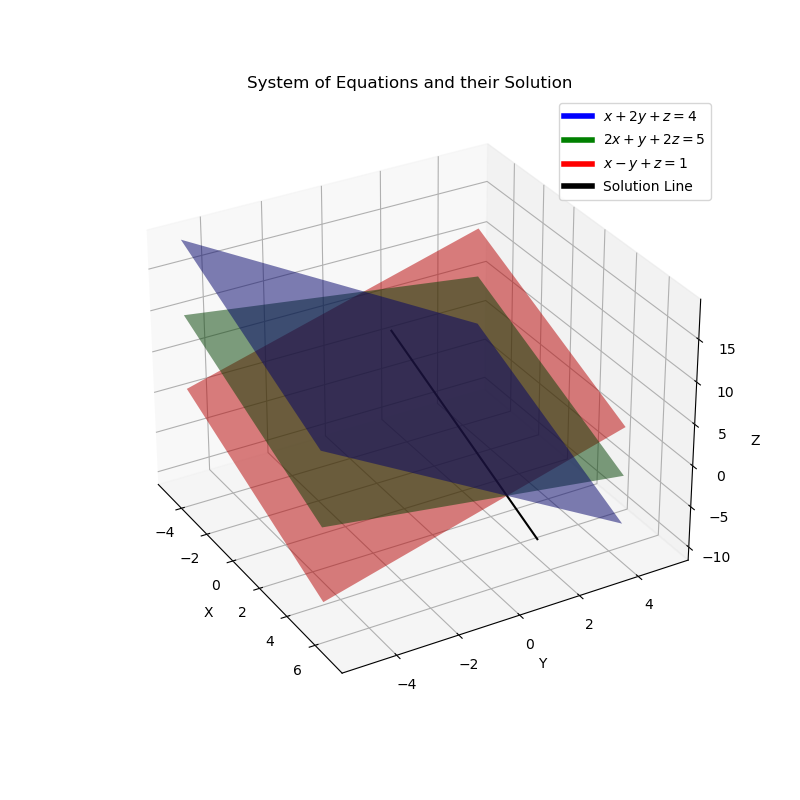
\includegraphics[width=0.64\linewidth]{figs/01.png}
   \caption{Plot of system of equations and solution line}
   \label{Plot_1}
\end{figure}
\end{document}
